\documentclass[a4paper,AutoFakeBold={2.7},UTF8,zihao=5,twoside]{ctexart} %纸张大小A4，文本类型为ctexart

%--------------------模板导言区：加载宏包，改变全局设置等--------------------%
\usepackage[colorlinks=true,urlcolor=black,linkcolor=black,citecolor=black]{hyperref}%超链接宏包,消除外部网址链接，文内交叉引用链接，参考文献引用链接的方框，且将字色改为黑
\usepackage{mathtools}%数学公式排版宏包
\usepackage{amssymb}%数学字体宏包
\usepackage{bbm}%提供\mathbbm字体
\usepackage{bm}%公式加粗宏包
\usepackage{arydshln}%分块矩阵宏包
\usepackage{fontspec}%字体设置宏包

\ctexset{section={format={\songti \zihao{-2} \bfseries \centering},beforeskip = 0.5\baselineskip,afterskip = 0.5\baselineskip,},%section样式设置
subsection={format={\songti \zihao{5} \bfseries},beforeskip=0pt,afterskip=0pt},%subsection样式设置
subsubsection={format={\songti \zihao{5} \bfseries},beforeskip=0pt,afterskip=0pt}} %subsubsection样式设置
\setmainfont{Times New Roman}%英文设置为Times New Roman
\renewcommand{\baselinestretch}{1.5}%改变默认行距为1.5倍行距

\usepackage{parskip}%智能段落间距宏包
\setlength{\parindent}{2em}  % 设置首行缩进为2个汉字宽度

\usepackage{mathrsfs}%允许使用\mathscr字体(花体字母)
\DeclareFontFamily{U}{rsfs}{\skewchar\font127 }% 手动配置 rsfs 字体族，确保在不同字号下使用正确的光学尺寸字体文件
\DeclareFontShape{U}{rsfs}{m}{n}{%
  <-6> rsfs5% <-6> rsfs5: 小于6pt使用rsfs5
  <6-8> rsfs7% <6-8> rsfs7: 6-8pt使用rsfs7
  <8-> rsfs10% <8-> rsfs10: 大于等于8pt使用rsfs10
}{}

\usepackage{booktabs}%三线表宏包
\usepackage{array}%表格宏包

\usepackage{tabularray}%跨页表格宏包
\UseTblrLibrary{booktabs} % 使用 booktabs 风格的线
\DefTblrTemplate{contfoot-text}{default}{\small 接下页}%跨页时，底部的字
\SetTblrTemplate{contfoot-text}{default}
\DefTblrTemplate{caption-sep}{default}{\ }%修改分隔符模板，将默认的冒号(:)改为空格
\SetTblrStyle{caption-tag}{font=\small\bfseries\heiti}%设置“表号”（如表1）的字体
\SetTblrStyle{caption-text}{font=\small\bfseries\heiti}%设置“标题内容”的字体
\DefTblrTemplate{conthead}{default}{}%将跨页后的标题区域设置为空
\SetTblrTemplate{conthead}{default}%应用设置，隐藏跨页后的表头
\DefTblrTemplate{capcont}{default}{}%将跨页后的表号（如“表1（续）”）设置为空
\SetTblrTemplate{capcont}{default}%应用设置

\usepackage{caption}%题注设置宏包
\DeclareCaptionFont{songti}{\songti}%为caption宏包定义heiti命令
\DeclareCaptionFont{wuhao}{\zihao{5}}%为caption宏包定义wuhao命令
\captionsetup{labelsep=space,font={wuhao,bf,songti},skip=5pt}%题注设置

\usepackage{graphicx}%图片宏包
\usepackage{float}%浮动体宏包，强制让浮动体在Here位置
\usepackage{subcaption}%子图宏包
\usepackage[left=2.5cm,right=2.5cm,top=2.5cm,bottom=2.5cm,includefoot]{geometry}%页边距设置

\usepackage{fancyhdr} % 引入页眉页脚宏包
% 设置页眉页脚样式
\pagestyle{fancy}
\fancyhf{} % 清空默认的页眉和页脚

% --- 核心：奇偶页眉设置 ---
% 偶数页
\fancyhead[CE]{偶数页页眉} 

% 奇数页
\fancyhead[CO]{奇数页页眉} 

% --- 底部页码 ---
\fancyfoot[C]{\thepage} % 底部居中显示页码

\fancypagestyle{headonly}{
  \fancyfoot{} % 这一句的作用是单独清空页脚
  % 至于页眉，它会自动继承你之前写好的 fancy 奇偶页眉设置
}

\setlength{\headheight}{14pt}%页眉高度稍微调大一点

\raggedbottom %取消文字必须强制贴齐纸张底部

\usepackage{wrapfig}%图片文字环绕宏包
\usepackage{xcolor}%颜色处理宏包
\usepackage{tcolorbox}%用于绘制带有背景色、圆角、边框的彩色盒子。
\usepackage{listings}%代码高亮宏包
\usepackage{ulem}%文本下划线与删除线宏包

% 加载 tcolorbox 的官方扩展库，：
% 1. listings: 将底层的 listings 代码排版功能与 tcolorbox 结合，允许你在漂亮的盒子里直接渲染带语法高亮的代码(解锁 \begin{tcblisting} 环境)。
% 2. skins: 加载高级皮肤引擎(基于 TikZ)，解锁更多高级视觉效果，例如阴影、渐变色、无缝拼接以及更复杂的圆角/边框样式。
% 3. breakable: 允许分页。
\tcbuselibrary{listings, skins, breakable}

% 定义类似 GitHub 的浅灰色背景和边框颜色
\definecolor{codegray}{HTML}{F6F8FA}
\definecolor{framegray}{HTML}{D1D5DA}
\definecolor{keywordcolor}{HTML}{005CC5}
\definecolor{stringcolor}{HTML}{032F62}
\definecolor{commentcolor}{HTML}{6A737D}

\setmonofont{Consolas}%设置给代码环境用的等宽字体

% 定义一个新的环境：code
\newtcblisting{code}[1][]{
  listing only,
  breakable,
  colback=codegray,        % 背景色
  colframe=framegray,      % 边框色
  boxrule=1pt,             % 边框粗细
  arc=3pt,                 % 圆角大小
  outer arc=3pt,
  left=4pt, right=4pt, top=2pt, bottom=2pt, % 内部边距
  listing options={
	mathescape=true,%允许注释使用latex公式
    basicstyle=\ttfamily\small, % 等宽字体和小字号
    breaklines=true,            % 自动换行
    keywordstyle=\color{keywordcolor}\bfseries,
    stringstyle=\color{stringcolor},
    commentstyle=\color{commentcolor},
    showstringspaces=false,
    language=#1,% 允许传入语言参数
  }
}

\usepackage[ruled,vlined,linesnumbered]{algorithm2e}%中文友好的算法环境
\renewcommand{\algorithmcfname}{算法}%algorithm2e 中文化
\SetKwInput{KwIn}{输入}
\SetKwInput{KwOut}{输出}
\SetKwRepeat{Repeat}{重复}{直到}

\numberwithin{equation}{section}%公式按章节编号

%--------------------项目导言区--------------------%
%加入本项目中要使用的宏包

%---------------------------标题、作者、日期---------------------------%
\title{\heiti \zihao{-2}\LaTeX 自制模板}%题目，黑体字，小二号大小
\author{\kaishu \zihao{-4}TYH\\ \songti \zihao{-5} 此处是作者简介:Ningbo University,226002262,major in mathmatic and applied mathmatic}%作者，楷体字，小四大小，作者简介宋体字，小五大小
\date{}%日期

%-----------------------------正文开始---------------------------------%
\begin{document}%开始

%-----------------------------封面---------------------------------%
\thispagestyle{empty}%封面不需要页码页眉
\vspace*{-3cm}

\begin{figure}[htbp]
    \centering
    
\includegraphics[width=0.7\textwidth]{配图/封面校徽.pdf}
\end{figure}

\vspace{-2cm}

\begin{center}
	\kaishu\zihao{-2}\bfseries 封面标题
\end{center}

\vspace{1cm}

\begin{center}
	\zihao{-2}\songti\bfseries 你的论文题目
\end{center}

\begin{center}
	\zihao{-2}\bfseries Your Thesis Title
\end{center}

\vspace{2cm}

\begin{center}
	\zihao{-3}
	学\qquad 院：\uline{\makebox[8cm][c]{\bfseries\songti 你的学院}} \\
	专\qquad 业：\uline{\makebox[8cm][c]{\bfseries\songti 你的专业}}\\
	班\qquad 级：\uline{\makebox[8cm][c]{\bfseries\songti 你的班级}}\\
	学\qquad 号：\uline{\makebox[8cm][c]{\bfseries\songti 你的学号}} \\
	学生姓名：\uline{\makebox[8cm][c]{\bfseries\songti 你的姓名}} \\
	指导教师：\uline{\makebox[8cm][c]{\bfseries\songti 你的导师}} \\
	完成时间：\uline{\makebox[8cm][c]{\bfseries\songti 你的日期}}
\end{center}

\clearpage

%-----------------------------诚信承诺书---------------------------------%
\thispagestyle{headonly}
\begin{center}
	{\kaishu\zihao{-2}\bfseries\ziju{1.5} 诚信承诺}
\end{center}

\vspace{1cm}

{\ziju{0.2}我谨在此承诺：本人所写的毕业论文《你的题目》的主体均系本人独立完成，没有抄袭行为，凡涉及其他作者的观点和材料，均作了注释，若有不实，后果由本人承担并自愿接受校方的处分。}

\vspace{1cm} % 和正文稍微空开一点点距离（可根据喜好调整）
\noindent\hfill % \hfill 就像一个横向的弹簧，把后面的表格挤到页面最右边
\begin{tabular}{ll}
	\kaishu\bfseries 承诺人（签名）：& \quad \\[0.5cm]
    & \kaishu\bfseries 年 \quad \kaishu\bfseries 月 \quad \kaishu\bfseries 日
\end{tabular}

\clearpage

%-----------------------------目录---------------------------------%
\pagenumbering{roman}%从目录开始到摘要页码用罗马数字编号
\begin{center}
	\tableofcontents%生成目录并居中，目录往往要编译两次才会正确显示
\end{center}

\clearpage

%-----------------------------中文摘要---------------------------------%
\renewcommand{\abstractname}{\bfseries\songti\zihao{-2}摘\qquad \bfseries\songti\zihao{-2}要}

\begin{center}
	\songti\zihao{-2}\bfseries 你的论文题目
\end{center}

\vspace{1cm}

\begin{abstract}
	\fangsong\zihao{-5}【{\bfseries\songti 摘要}】你的摘要

	\vspace{12pt}

	\noindent【{\songti\bfseries 关键词}】你的关键词1；你的关键词2；你的关键词3；你的关键词4
\end{abstract}
\clearpage

%-----------------------------英文摘要---------------------------------%
\renewcommand{\abstractname}{\zihao{-2}\bfseries Abstract}

\begin{center}
	\zihao{-2}\bfseries Your Thesis Title
\end{center}

\vspace{1cm}

\begin{abstract}
	\zihao{-5}【\textbf{ABSTRACT}】Your Abstract

	\vspace{12pt}

	\noindent【\textbf{KEYWORDS}】Your Keyword 1; Your Keyword 2; Your Keyword 3; Your Keyword 4
\end{abstract}
\clearpage

\pagenumbering{arabic}%正文页码用阿拉伯数字编号

\section{第一节一级标题}%第一节一级标题
内容1
\subsection{第一节二级标题} \label{第一节二级标题}
内容1.1
\subsubsection{第一节三级标题}
内容1.1.1
\subsection{假设}
(1)假设一：

(2)假设二：

\clearpage

\section{第二节一级标题}
内容2
\subsection{第二节二级标题}
内容2.1
\subsubsection{第二节三级标题}
内容2.1.1
\subsection{第二节二级标题}
内容2.2

\clearpage

\section{图片插入}
一张图中可以只有一张子图，也可以由多个子图构成一张图。
\subsection{单个子图}

\begin{figure}[H]%H代表强制在Here位置
	\centering
	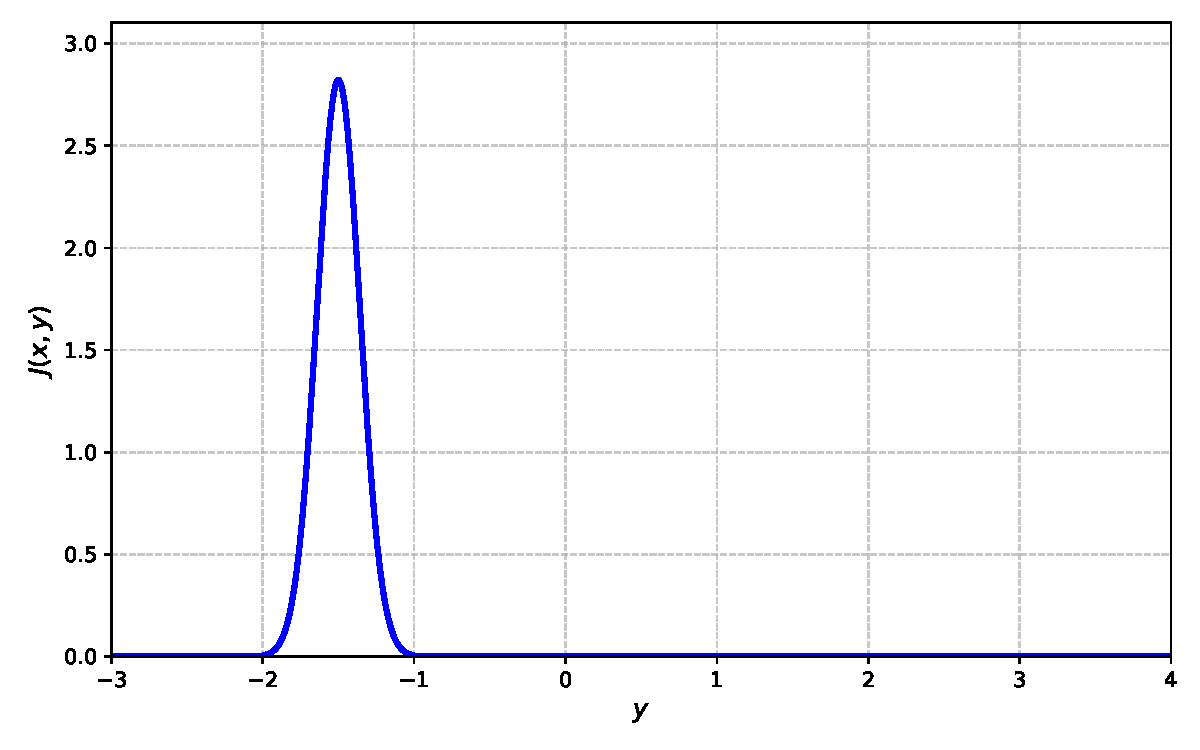
\includegraphics[width=0.5\linewidth]{配图/时谐电流源J.pdf}
	\caption{图名}\label{图名}
\end{figure}

\subsection{多个子图(以2×2子图为例)}

\begin{figure}[H]
    \centering
    % 第一行
    \begin{subfigure}[b]{0.45\textwidth}%[b]表示这一行所有子图的底部边缘(通常是子图标题的最后一行水平基线)对齐在同一条水平线上。这是学术排版中最常用、看起来最整齐的设置。
        \centering
        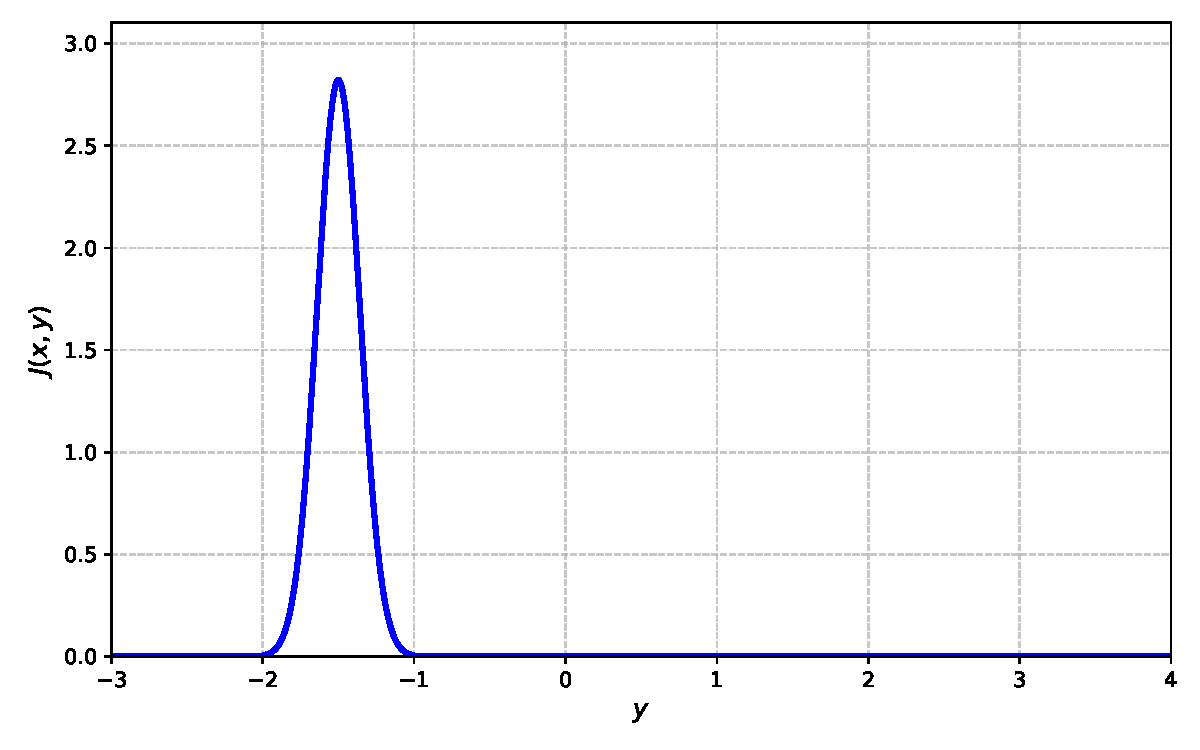
\includegraphics[width=\textwidth]{配图/时谐电流源J.pdf}
        \caption{SubFigure1}
        \label{fig:sub1}
    \end{subfigure}
    \hfill % 使用 hfill 自动推开间距，比手动 hspace 更好控制
    \begin{subfigure}[b]{0.45\textwidth}
        \centering
        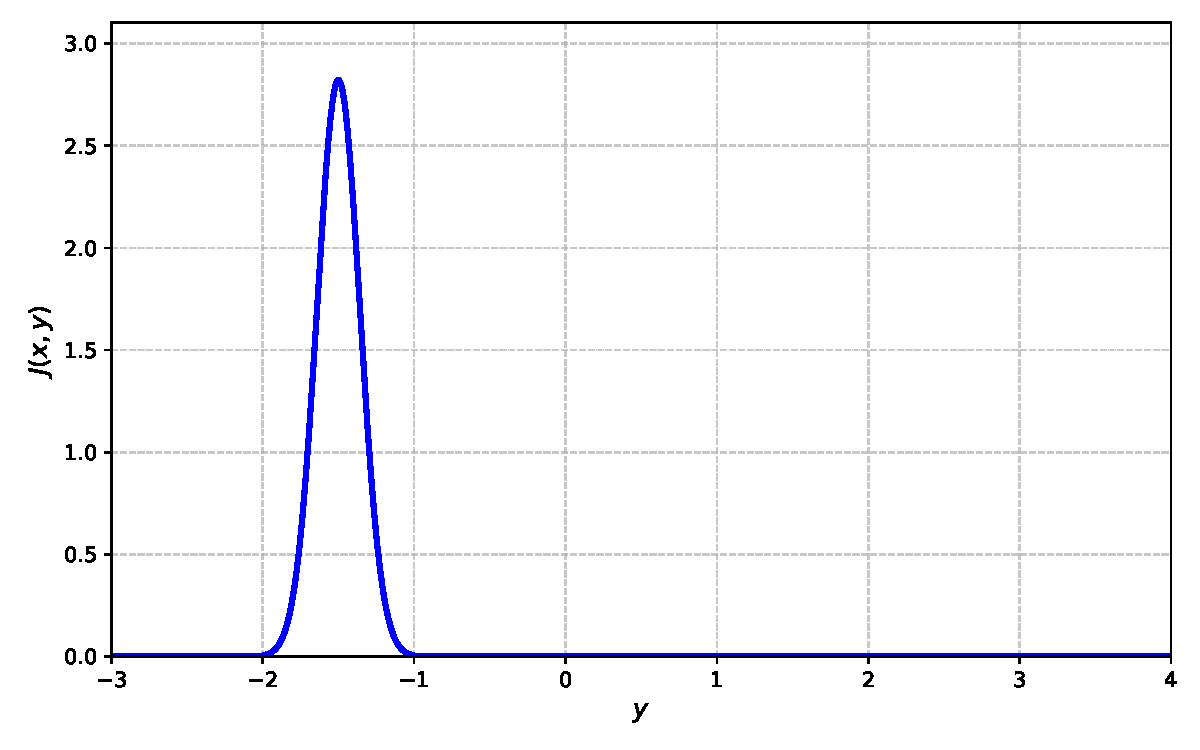
\includegraphics[width=\textwidth]{配图/时谐电流源J.pdf}
        \caption{SubFigure2}
        \label{fig:sub2}
    \end{subfigure}
    
    \vspace{0.3cm} % 第一行和第二行之间的垂直间距

    % 第二行
    \begin{subfigure}[b]{0.45\textwidth}
        \centering
        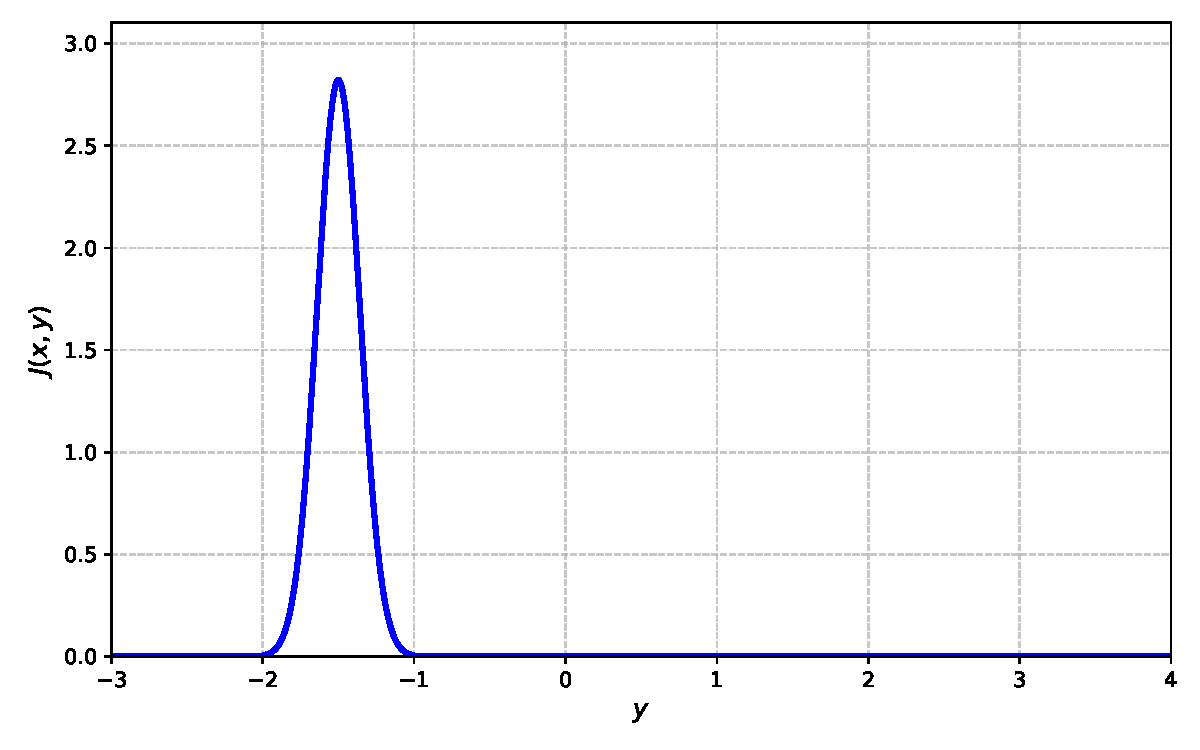
\includegraphics[width=\textwidth]{配图/时谐电流源J.pdf}
        \caption{SubFigure3}
        \label{fig:sub3}
    \end{subfigure}
    \hfill
    \begin{subfigure}[b]{0.45\textwidth}
        \centering
        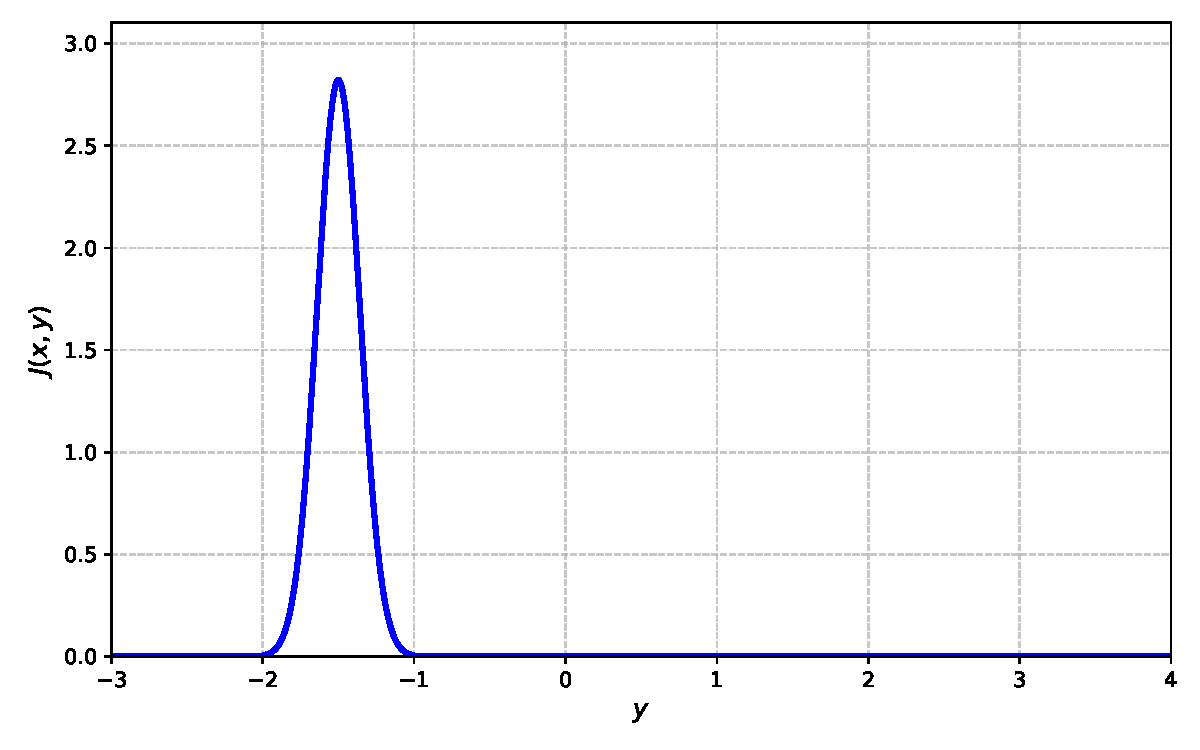
\includegraphics[width=\textwidth]{配图/时谐电流源J.pdf}
        \caption{SubFigure4}
        \label{fig:sub4}
    \end{subfigure}
    
    \caption{2×2布局}
    \label{fig:main}
\end{figure}

\clearpage

\section{表格插入}
表格有普通的单页表格和长度较大的跨页表格
\subsection{单页表格}
首先展示单页表格：

\begin{table}[htbp]%h:here当前位置,t:top页面顶部,b:bottom页面底部,p:page另放一页
	\caption{表名}\label{表名}
	\centering
	\begin{tabular}{p{3cm}<{\centering} p{3cm}<{\centering} p{3cm}<{\centering} p{3cm}<{\centering}}
		%p{3cm}规定列宽，\centering规定居中对其
		\toprule[1.5pt]
		1&2&3&4\\
		\midrule[0.75pt]
		内容&内容&内容&内容\\
		内容&内容&内容&内容\\
		内容&内容&内容&内容\\
		\bottomrule[1pt]
	\end{tabular}
\end{table}

\subsection{跨页表格}
展示跨页表格：

\begin{longtblr}[
	caption={数据缺失值统计表},
	label={数据缺失值统计表},
	]{
		% 列定义：Q类型，c=居中，4cm宽度
		colspec = {Q[c,4cm] Q[c,4cm] Q[c,4cm]}, 
		% 线条设置：使用 booktabs 风格
		hline{1,Z} = {1pt},   % 第一行顶端(1)和最后一行底端(Z) 加粗线
		hline{2}   = {0.5pt}, % 第一行下面(即表头下) 加细线
		rowhead = 1, % 将第1行设为表头，跨页时自动重复
}
    %表格内容
    列名 & 非空单元格数量 & 数据类型 \\ % 这是第1行，会被自动作为表头
    customerID        & 7043 & object  \\
    gender            & 7043 & object  \\
    SeniorCitizen     & 7043 & int64   \\
    Partner           & 7043 & object  \\
    Dependents        & 7043 & object  \\
    tenure            & 7043 & int64   \\
    PhoneService      & 7043 & object  \\
    MultipleLines     & 7043 & object  \\
    InternetService   & 7043 & object  \\
    OnlineSecurity    & 7043 & object  \\
    OnlineBackup      & 7043 & object  \\
    DeviceProtection  & 7043 & object  \\
    TechSupport       & 7043 & object  \\
    StreamingTV       & 7043 & object  \\
    StreamingMovies   & 7043 & object  \\
    Contract          & 7043 & object  \\
    PaperlessBilling  & 7043 & object  \\
    PaymentMethod     & 7043 & object  \\
    MonthlyCharges    & 7043 & float64 \\
    TotalCharges      & 7043 & object  \\
    Churn             & 7043 & object  \\
    Churn             & 7043 & object  \\
    Churn             & 7043 & object  \\
    Churn             & 7043 & object  \\
    Churn             & 7043 & object  \\
    Churn             & 7043 & object  \\
    Churn             & 7043 & object  \\
    Churn             & 7043 & object  \\
    Churn             & 7043 & object  \\
\end{longtblr}

\clearpage

\section{数学公式}
\subsection{行内公式}
行内公式，$a+b=c$，希腊字母$\alpha\beta\gamma$，定积分$\int_{a}^{b} f(x)dx$，不定积分$\int f(x)dx$，
\subsection{行间公式}
\begin{equation}
	S_{n}=\sum_{k=1}^{n} x_{k} \label{(1)}
\end{equation}
\begin{equation}
	\alpha\left( x+y\right) =z
\end{equation}
方程组：
\begin{equation}
	\begin{cases}
		x_{1}^{2}+y_{1}^2=a\\
		x_{1}-y_{1}=b\\
		x_{1}+y_{1}=c
	\end{cases}
\end{equation}
分段函数：
\begin{equation}
	f(x)=
	\begin{cases}
		f_{1}(x) &x>a\\
		f_{2}(x) &x<=a
	\end{cases}
\end{equation}
长公式：
\begin{equation}
	\begin{split}
		f(x)&=1000000a+2000000b+30000c+400000d\\
		&=1000000\alpha+200000\beta+3000000\gamma+40000\delta\\
		&=\zeta+\eta+\theta+\lambda
	\end{split}
\end{equation}

普通矩阵
\begin{equation}
	\begin{bmatrix}
		\varphi\\
		\theta\\
		\psi
	\end{bmatrix}
	=
	\begin{bmatrix}
		a_{11} & a_{12} & a_{13} \\
		a_{21} & a_{22} & a_{23} \\
		a_{31} & a_{32} & a_{33}
	\end{bmatrix}
	\begin{bmatrix}
		x_{1} \\
		x_{2} \\
		x_{3}
	\end{bmatrix}
\end{equation}

高维矩阵
\begin{equation}
	\begin{bmatrix}
		a_{11} & a_{12} & \cdots & a_{1n} \\
		a_{21} & a_{22} & \cdots & a_{2n} \\
		\vdots & \vdots & \ddots & \vdots \\
		a_{n1} & a_{n2} & \cdots & a_{nn}
	\end{bmatrix}
\end{equation}

行列式：
\begin{equation}
  \begin{vmatrix}
    f_1(a_1) & f_1(a_2) & \cdots & f_1(a_n) \\
    f_2(a_1) & f_2(a_2) & \cdots & f_2(a_n) \\
    \vdots   & \vdots   &        & \vdots   \\
    f_n(a_1) & f_n(a_2) & \cdots & f_n(a_n)
  \end{vmatrix}
  = 0
\end{equation}

\clearpage

\section{算法示例}

\begin{algorithm}
\caption{累加求和算法}
\KwIn{正整数 $n$}
\KwOut{$1$ 到 $n$ 的和}

初始化 $s \gets 0$\;
\For{$i = 1$ \KwTo $n$}{
    $s \gets s + i$\;
}
\Return $s$\;
\end{algorithm}

\clearpage

%-------------------------------致谢-----------------------------%
\begin{center}
	\zihao{-3}\songti\bfseries 致\quad 谢
\end{center}

你的致谢

\clearpage

%-------------------------------参考文献-----------------------------%
\begingroup% 临时强制让 section 标题居中
\ctexset{section/format={\centering\songti\zihao{-2}\bfseries}}
\begin{thebibliography}{99}
	\addcontentsline{toc}{section}{参考文献}%将参考文献添加到目录中
	\bibitem{参考文献1}这是参考文献1
	
	\bibitem{参考文献2}这是参考文献2
	
	\bibitem{参考文献3}这是参考文献3
\end{thebibliography}
\endgroup

%--------------------------------附录--------------------------------%
\appendix
\ctexset{
  section = {
    number = \Alph{section},
    name = {附录}
  }
}%设置附录部分的一级标题格式

\section{引用测试}

外部网址链接：\url{www.bing.com}

文内交叉引用测试：\ref{第一节二级标题}

公式引用测试\ref{(1)}

脚注测试\footnote{这是脚注}

表格引用测试 表\ref{表名}

图片引用测试 图\ref{图名}

参考文献测试\textsuperscript{\cite{参考文献1}}

参考文献测试\textsuperscript{\cite{参考文献1}\cite{参考文献2}}

\clearpage

\section{附录公式}

高维矩阵
\begin{equation}
	\begin{bmatrix}
		a_{11} & a_{12} & \cdots & a_{1n} \\
		a_{21} & a_{22} & \cdots & a_{2n} \\
		\vdots & \vdots & \ddots & \vdots \\
		a_{n1} & a_{n2} & \cdots & a_{nn}
	\end{bmatrix}
\end{equation}

行列式：
\begin{equation}
  \begin{vmatrix}
    f_1(a_1) & f_1(a_2) & \cdots & f_1(a_n) \\
    f_2(a_1) & f_2(a_2) & \cdots & f_2(a_n) \\
    \vdots   & \vdots   &        & \vdots   \\
    f_n(a_1) & f_n(a_2) & \cdots & f_n(a_n)
  \end{vmatrix}
  = 0
\end{equation}

\clearpage

\section{附录代码}

\begin{code}[Python]
# 这是一段 Python 代码演示
def fetch_data(url):
    """
    Fetch data from the given URL.
    """
    message = "Loading data..."
    print(message)
    return {"status": 200, "data": [1, 2, 3]}
\end{code}

\end{document}%结束